%!TEX root = ./paper.tex

\section*{Appendix}

\begin{figure}[h]
  \centering 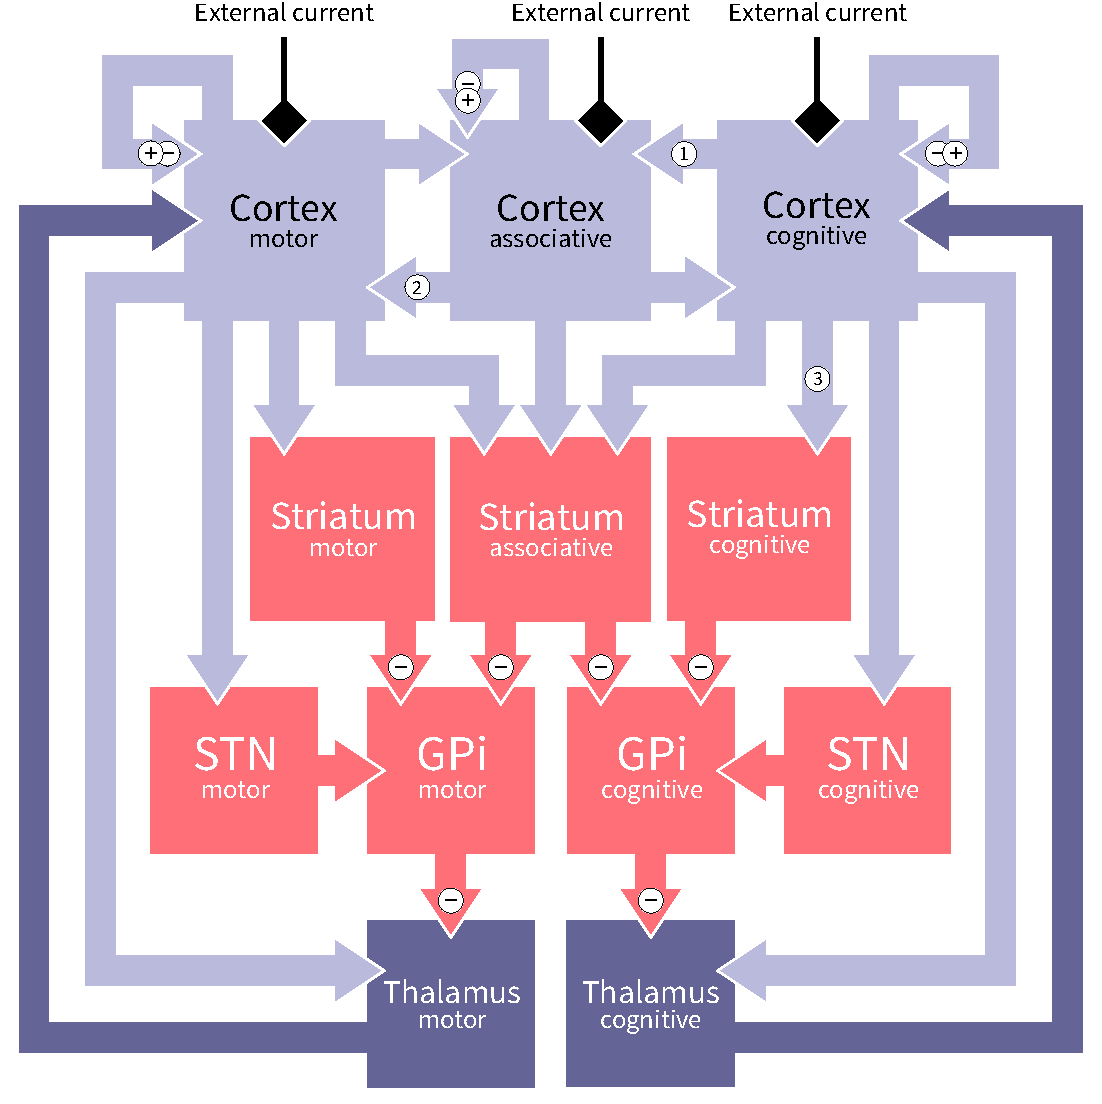
\includegraphics[width=0.5\textwidth]{architecture}
  \caption{Architecture of the model: Display of the connections
  					among the nuclei through the direct pathway
  					(Cortex-Striatum-GPi-Thalamus-Cortex) and
  					hyperdirect (Cortex-Striatum-GPi-Thalamus-Cortex).
  					Learning occurs in two levels: hebbian learning
  					 at the cortical through connections (1) and 
  					 reinforcement learning at striatal through connections 
  					 (3).}
  \label{fig:architecture}
\end{figure}



\begin{figure}[h]
        \centering
        \begin{subfigure}[b]{0.4\textwidth}
                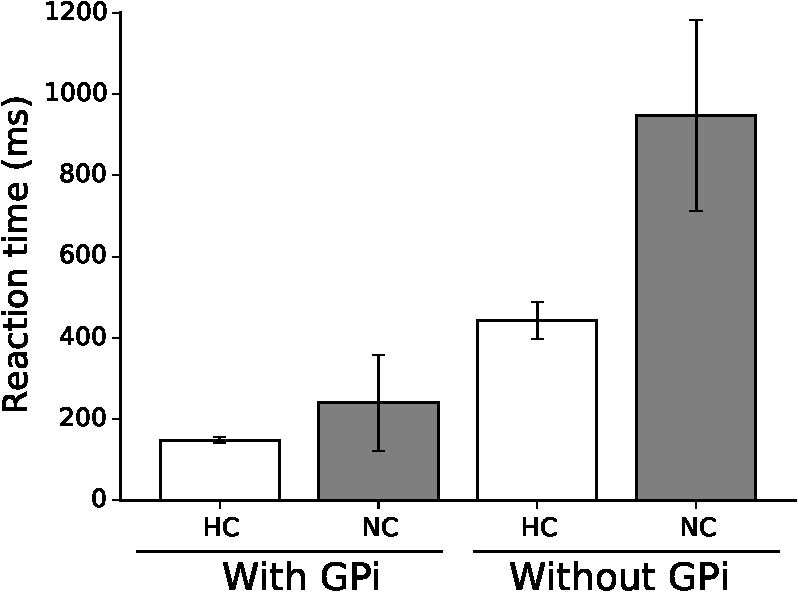
\includegraphics[width=\textwidth]{RTresults}
                
        		  \vspace{2mm}
                \caption{Reaction time of the model}
                \label{fig:RTresults}
        \end{subfigure}
        \vspace{4mm}
        
        \begin{subfigure}[b]{0.9\textwidth}
                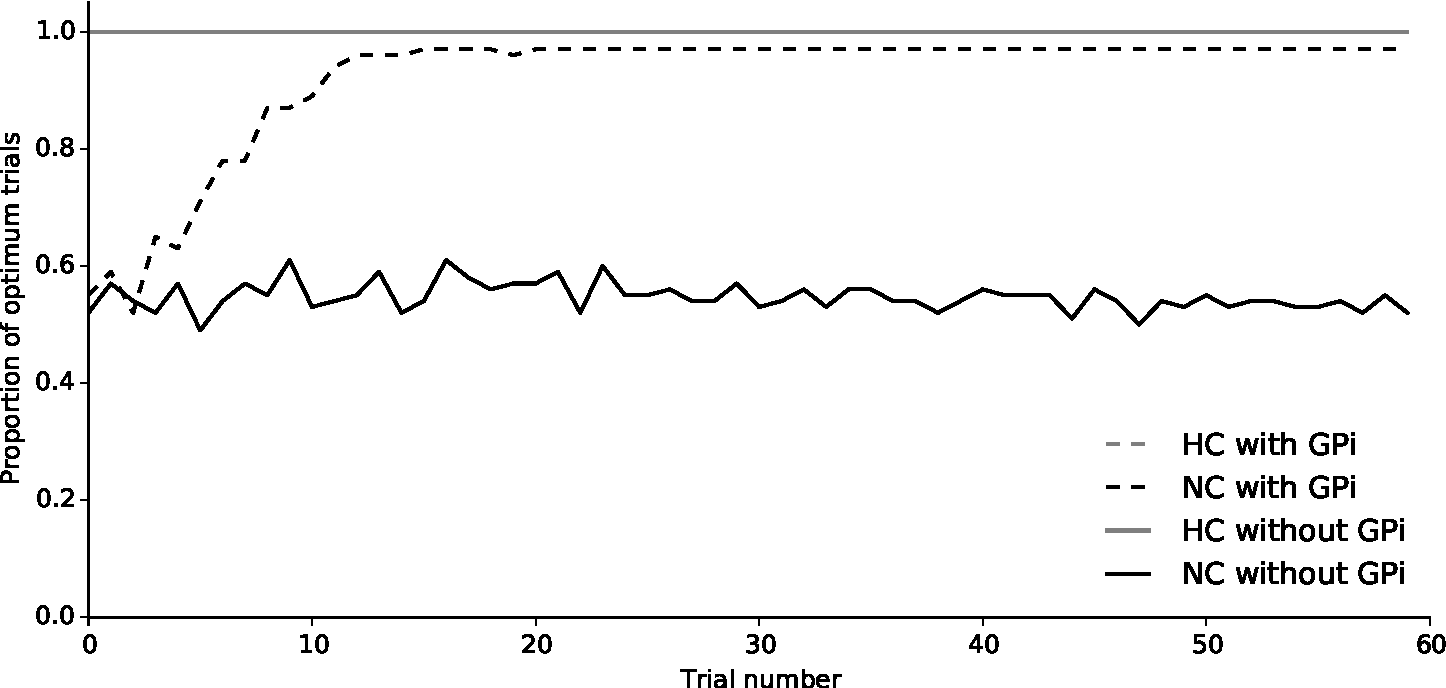
\includegraphics[width=\textwidth]{Performances}
        		  \vspace{2mm}
                \caption{Performances of the model}
                \label{fig:Performances}
        \end{subfigure}
        \vspace{4mm}
        \caption{Results of the model: 
        					\ref{fig:RTresults}) Analysis of the data showed that
        					 reaction time is higher in NC as compared to HC 
        					 with active and inactive GPi. The later increases
        					 significantly the reaction time in both conditions.
        					 \ref{fig:Performances}) In HC, the choice of the
        					 optimal target is made always with and without
        					 GPi. This is not the case in NC. With active GPi, the
        					 choice at the beginning is random, but finally there 
        					 is expression of preference to the optimal target. 
        					 Contrary, the choice continues to be random for the
        					 case of inactive GPi.}
\end{figure}

